\documentclass[oneside, 11pt]{article}

\usepackage[T1]{fontenc}
\usepackage[utf8]{inputenc}
\usepackage[english]{babel}

\usepackage{fouriernc}
\usepackage[detect-all, binary-units, separate-uncertainty=true,
            per-mode=symbol, retain-explicit-plus, retain-unity-mantissa=false]{siunitx}

\usepackage{setspace}
\setstretch{1.2}

\setlength{\parskip}{\smallskipamount}
\setlength{\parindent}{0pt}

\usepackage[headheight=14pt]{geometry}
\geometry{marginparwidth=0.5cm, verbose, a4paper, tmargin=3cm, bmargin=3cm,
          lmargin=2cm, rmargin=2cm}

\usepackage{float}

\usepackage[fleqn]{amsmath}
\numberwithin{equation}{section}
\numberwithin{figure}{section}

\usepackage{graphicx}
\graphicspath{{images/}{../../../images/}}

\usepackage{tikz}
\usetikzlibrary{shapes}
\usetikzlibrary{plotmarks}

\newcounter{Exercise}
\setcounter{Exercise}{1}
\usepackage{xcolor}
\definecolor{shadecolor}{gray}{0.9}
\usepackage{framed}
\usepackage{caption}

\usepackage{url}


\usepackage{fancyhdr}
\pagestyle{fancy}
\fancyhf{}
\rhead{\thepage}
\renewcommand{\footrulewidth}{0pt}
\renewcommand{\headrulewidth}{0pt}

\fancypagestyle{firststyle}
{
    \fancyhf{}
    \rhead{\thepage}
    \cfoot{
\includegraphics[height=30pt]{HiSPARClogo}}
    \rfoot{
\includegraphics[height=25pt]{CCbysa}}
    \lfoot{
\includegraphics[height=30pt]{NIKHEFlogo}}
    \renewcommand{\footskip}{50pt}
    \renewcommand{\footrulewidth}{0.1pt}
    \renewcommand{\headrulewidth}{0pt}
}

\newcommand{\figref}[1]{Figuur~\ref{#1}}

\newcommand{\hisparc}{\textsmaller{HiSPARC}\xspace}
\newcommand{\kascade}{\textsmaller{KASCADE}\xspace}
\newcommand{\sapphire}{\textsmaller{SAPPHiRE}\xspace}
\newcommand{\jsparc}{\textsmaller{jSparc}\xspace}
\newcommand{\hdf}{\textsmaller{HDF5}\xspace}
\newcommand{\aires}{\textsmaller{AIRES}\xspace}
\newcommand{\csv}{\textsmaller{CSV}\xspace}
\newcommand{\python}{\textsmaller{PYTHON}\xspace}
\newcommand{\corsika}{\textsmaller{CORSIKA}\xspace}
\newcommand{\labview}{\textsmaller{LabVIEW}\xspace}
\newcommand{\daq}{\textsmaller{DAQ}\xspace}
\newcommand{\adc}{\textsmaller{ADC}\xspace}
\newcommand{\hi}{\textsc{h i}\xspace}
\newcommand{\hii}{\textsc{h ii}\xspace}
\newcommand{\mip}{\textsmaller{MIP}\xspace}
\newcommand{\hisparcii}{\textsmaller{HiSPARC II}\xspace}
\newcommand{\hisparciii}{\textsmaller{HiSPARC III}\xspace}

\DeclareSIUnit{\electronvolt}{\ensuremath{\mathrm{e\!\!\:V}}}

\DeclareSIUnit{\unitsigma}{\ensuremath{\sigma}}
\DeclareSIUnit{\mip}{\textsmaller{MIP}}
\DeclareSIUnit{\adc}{\textsmaller{ADC}}

\DeclareSIUnit{\gauss}{G}
\DeclareSIUnit{\parsec}{pc}
\DeclareSIUnit{\year}{yr}




%document details
\author{N.G. Schultheiss \\ translated and adapted by K. Schadenberg}
\date{}
\title{Cherenkov}


\begin{document}
\maketitle

\section{Introduction}
This module follows the module `Compton'.

\section{Cherenkov}
Pavel Alekseyevich Cherenkov (1904-1990) was a Soviet physicist who shared the Nobel Prize in Physics in 1958 with Ilya Frank and Igor Tamm for the discovery of Cherenkov radiation made in 1934.

Cherenkov was researching the radiation emitted by nuclear reactors containing water which is used both as a cooling agent as well as a neutron moderator.\footnote{A moderator is a medium that reduces the speed of fast neutrons inside nuclear reactors. This deceleration is necessary to maintain the nuclear reaction. Without the moderator the fast neutrons will escape the reactor vessel without interacting with other nuclei. This will cause the reactor to shut down. Too many slow neutrons is also a problem. A rapid increase in the number of nuclear reactions causes overheating. If this is not stopped soon enough the reactor could be damaged by a melt-down (Harrisburg and Chernobyl).}

As we have seen with the Geigercounter, moving particles can knock away electrons from a medium. The electron can jump to a higher energy state within the atom or be made completely free from the atom (also a form of higher energy state). With Cherenkov radiation the electron immediately returns to its ground state, emitting its excess energy in the form of a photon. If this happens in water then photons won't have the the speed of light in vacuum, but it will move slower:
\begin{equation*}
c_{medium} = \frac{c}{N_{medium}}
\end{equation*}
The particle that knocked the electron into a higher energy state could have had a higher velocity than $c_{medium}$.

Let us assume the particle was travelling faster than the speed of light in the medium. Just like a plane flying at supersonic speed, the particle will emit a cone of light (the plane `emits' a cone of sound). Because the particle scatters every time it hits an electron, this cone of light won't be very well defined. The emission of (visible) light is called Cherenkov radiation. Because lighter particles are scattered more easily, one can estimate the mass of the particle by looking at the `sharpness' of the light cone.

\begin{figure}\begin{center}
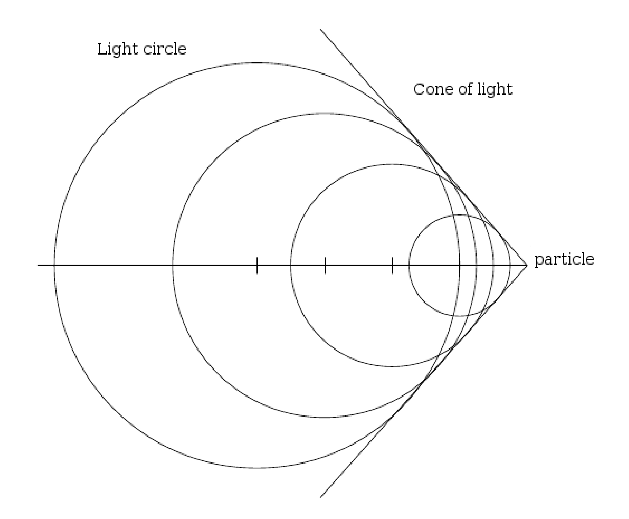
\includegraphics[scale=1]{light_cone_s}%
\caption{Schematic representation of the emission of Cherenkov radiation.}\label{fig:light_cone}
\end{center}\end{figure}

\end{document}